% Figure 5.2 (Session 5): the spinless chain as the XXZ chain, and charge order from a pinning field.
% The image is rendered by figures/blender/s5_2_xxz_pinning.py; the coordinates of the labels
% come from figures/blender/out/xxz_pinning_anchors.tex. Built by figures/blender/build_figure.sh.
\documentclass[11pt,tikz,border=0pt]{standalone}
\usepackage{amsmath,amssymb,graphicx,braket}
\usepackage{xcolor}
\definecolor{coursedark}{HTML}{1B2A4A}
\definecolor{costamber}{HTML}{B8620A}
\newlength{\figw}\setlength{\figw}{16.19cm}   % the text width of the notes (letter, 2.7 cm margins), so labels print at size

\begin{document}
\begin{tikzpicture}[lbl/.style={font=\small, text=coursedark}]
  \node[anchor=south west, inner sep=0pt] at (0,0)
    {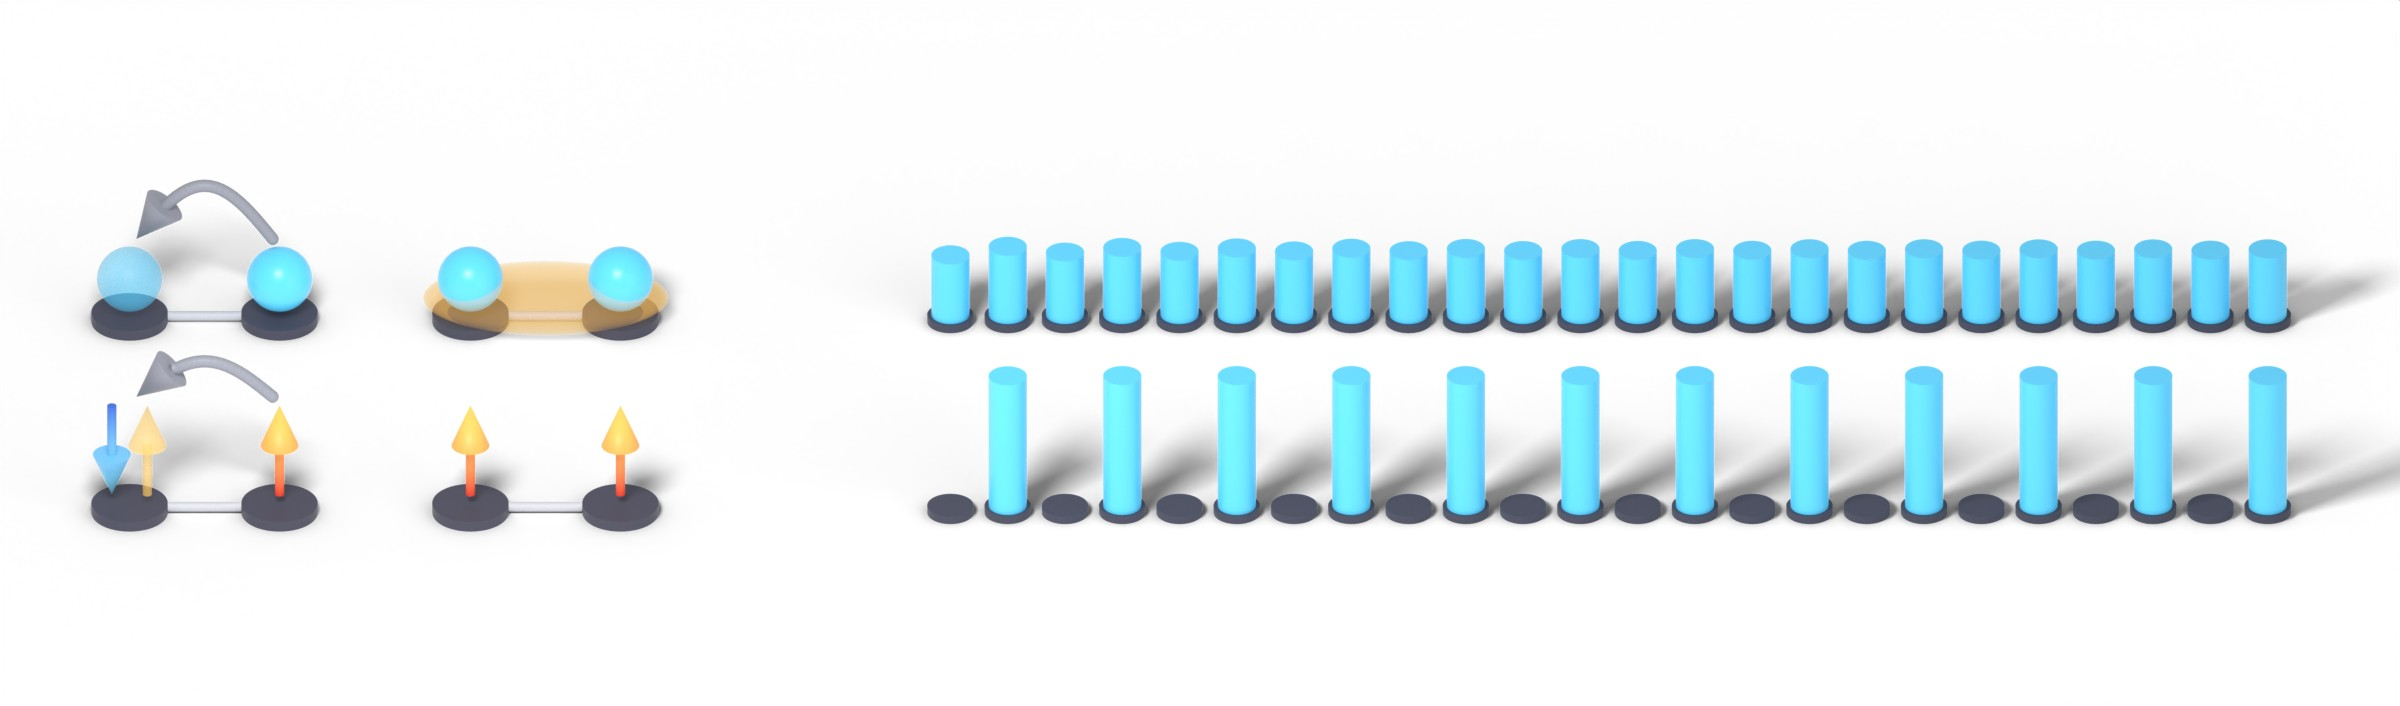
\includegraphics[width=\figw]{../blender/out/xxz_pinning.jpg}};
  %% written by figlib.py; x and y in units of the image width
\coordinate (tf) at (0.0852\figw,0.2266\figw);
\coordinate (ts) at (0.0852\figw,0.0650\figw);
\coordinate (Vf) at (0.2273\figw,0.2094\figw);
\coordinate (Vs) at (0.2273\figw,0.0650\figw);
\coordinate (a) at (0.0085\figw,0.2955\figw);
\coordinate (row0) at (0.3761\figw,0.1774\figw);
\coordinate (row1) at (0.3761\figw,0.0979\figw);
\coordinate (edge) at (0.3960\figw,0.0678\figw);
\coordinate (bulk) at (0.9449\figw,0.0678\figw);
\coordinate (b) at (0.3693\figw,0.2955\figw);

  \node[lbl, font=\normalsize, anchor=west] at (a) {(a)};
  \node[lbl, font=\normalsize, anchor=west] at (b) {(b)};
  \node[lbl, anchor=south] at (tf) {$-t\,c^\dagger_i c^{\phantom{\dagger}}_{i+1}$};
  \node[lbl, anchor=north] at (ts) {$-t\,S^+_i S^-_{i+1}$};
  \node[lbl, text=costamber, anchor=south] at (Vf) {$V n_i n_{i+1}$};
  \node[lbl, text=costamber, anchor=north] at (Vs) {$V S^z_i S^z_{i+1}+\dots$};
  \node[lbl, anchor=east] at (row0) {$V=t$};
  \node[lbl, anchor=east] at (row1) {$V=40t$};
  \node[lbl, anchor=north] at (edge) {edge};
  \node[lbl, anchor=north] at (bulk) {site 24 of 100};
\end{tikzpicture}
\end{document}
